\documentclass[11pt,a4paper]{article}

\usepackage[margin=2.5cm]{geometry}
\usepackage{graphicx}
\usepackage{booktabs}
\usepackage{array}
\usepackage{float}
\usepackage{natbib}
\usepackage{hyperref}
\hypersetup{
  colorlinks=true,
  citecolor=blue,
  linkcolor=blue,
  urlcolor=blue
}
\usepackage{xcolor}
\usepackage{tikz}
\usetikzlibrary{arrows.meta,positioning,fit,shapes.geometric}
\setlength{\parindent}{0pt}
\emergencystretch=3em

\title{GrapeMaster: An End-to-End Mobile Decision-Support Platform for Vineyard Disease Warning and Precision Management}
\author{Author information to be completed before submission}
\date{}

\begin{document}
\maketitle

\begin{abstract}
Timely grapevine disease management requires the integration of local weather, crop phenology, disease-risk modeling, field observations, and plant-protection records within operational decision workflows. This study developed GrapeMaster, an end-to-end mobile decision-support platform for vineyard disease warning and precision management. The platform uses the crop season as the central data unit to link vineyard fields, weather retrieval, phenology simulation, disease-risk prediction, spraying-suitability assessment, image-based disease assistance, notifications, field notes, and plant-protection tasks. The system was implemented with a Flutter mobile client, a Django REST backend, PostgreSQL storage, scheduled analytical workflows, a FastAPI disease-model service, and Python-based image-recognition and severity-estimation modules. A central design feature is the closed management loop in which model outputs are translated into warnings, treatment windows, and tasks, while completed fungicide applications are converted into history inputs for subsequent disease-risk recalculation. Initial deployment in Yangling, Nanning, Du'an, and Xing'an showed that spore detection preceded visible disease onset by approximately one to two months, and that model-guided spray timing was associated with at least three fewer fungicide applications per season than conventional grower practice. These results demonstrate the feasibility of using GrapeMaster to connect vineyard disease warning, mobile field operations, and management feedback, while multi-season validation, quantitative model evaluation, and user-centered assessment remain necessary for operational validation.
\end{abstract}

\textbf{Keywords:} precision viticulture; grapevine disease warning; mobile decision support; crop-season management; phenology simulation; disease-risk modeling; image-based diagnosis

\section{Introduction}

Plant pathogens and pests remain a major constraint on agricultural production, reducing both yield and quality and creating strong demand for timely, site-specific crop-health management \citep{Savary2019GlobalBurden}. Grapevine production is particularly exposed to disease risks because major foliar and fruit diseases, including downy mildew, powdery mildew, gray mold, and black rot, respond dynamically to local weather, host growth stage, cultivar susceptibility, canopy condition, and recent plant-protection operations \citep{Peng2024DownyMildew,Kunova2021PowderyMildew,Rahman2024GrayMold,Szabo2023BlackRot,Puelles2024DownyMildewModels}. Gray mold and other bunch rots affect grape and wine quality as well as yield, while powdery mildew and downy mildew management remains closely linked to fungicide timing and resistance-aware disease control \citep{Steel2013BunchRots,Kunova2021PowderyMildew,Peng2024DownyMildew}. In practice, disease control is also shaped by environmental and regulatory pressure to reduce unnecessary pesticide inputs while maintaining fruit quality and yield stability \citep{Mian2021DownyMildewDSS,Rossi2014ViteNet}. Disease management in vineyards is therefore a continuous decision process, not only a diagnostic problem, because growers must interpret infection-conducive weather, phenological susceptibility, visible symptoms, treatment windows, and fungicide protection history within a short operational period \citep{Orlandini1993PLASMO,Rossi2014ViteNet,Puelles2024DownyMildewModels}.

Several technical approaches have been developed to support this process, especially weather-driven disease models, phenological models, decision-support systems, and image-based diagnosis methods \citep{Orlandini1993PLASMO,Rossi2014ViteNet,OrtegaFarias2019Phenology,Xie2020GrapeDetector}. Weather-driven disease models have long been used to simulate pathogen development and guide fungicide timing in vineyards \citep{Orlandini1993PLASMO,Orlandini1995DownyMildewProgram}. For example, PLASMO simulated grapevine downy mildew development from temperature, leaf wetness, relative humidity, and treatment information, and was designed for direct use in vineyard management \citep{Orlandini1993PLASMO}. Later model-based systems and evaluations showed that downy mildew prediction remains sensitive to regional climatic conditions and therefore requires field-level calibration, validation, and operational interpretation rather than simple transfer of generic infection rules \citep{Orlandini1995DownyMildewProgram,Puelles2024DownyMildewModels}. Vineyard decision-support systems such as vite.net combined real-time monitoring, data storage, mechanistic models, alerts, and web-based decision support, explicitly addressing the implementation problem that has limited the sustained use of many agricultural DSSs \citep{Rossi2014ViteNet,McCown2002DSSComplexity,Rose2016DecisionSupportTools}. In parallel, grapevine growth-stage scales and phenology models provide a formal basis for linking crop development to management timing, including BBCH or modified Eichhorn-Lorenz stage descriptions and cumulative-degree-day model formulations \citep{Lorenz1995BBCH,Coombe1995ModifiedEL,OrtegaFarias2019Phenology,Molitor2014HighResolutionPhenology}. Recent cultivar-scale and multi-stage phenology models further indicate that temperature-driven development can be represented quantitatively across cultivars, although calibration data and regional context affect model behavior \citep{Caffarra2014PhenologyComparison,Molitor2020UniPhen,OrtegaFarias2019Phenology}.

Recent advances in computer vision have added another important source of field evidence for crop-health assessment \citep{Xie2020GrapeDetector,Liu2020GrapeLeafIdentification,Shi2023SeverityAssessment}. Deep convolutional networks, vision transformers, and object-detection models have been applied to grape leaf disease classification, downy mildew detection, and lesion localization under natural or semi-natural imaging conditions \citep{Xie2020GrapeDetector,Liu2020GrapeLeafIdentification,Zhang2022DownyMildewDetection,Kunduracioglu2024GrapeDeepLearning,Liu2024FusionTransformerYOLO}. Disease-severity studies further emphasize the value of pixel-level lesion and leaf segmentation for quantifying symptom intensity instead of reporting only a class label \citep{Shi2023SeverityAssessment}. These methods can reduce dependence on manual visual inspection and support fast symptom-level assessment in the field \citep{Xie2020GrapeDetector,Zhang2022DownyMildewDetection,Kunduracioglu2024GrapeDeepLearning}. However, image diagnosis alone does not explain whether weather and phenology are favorable for infection, whether a treatment window is open, or whether previous fungicide applications still provide protection, because those decisions depend on weather-driven epidemiology, growth stage, and treatment history \citep{Orlandini1993PLASMO,Rossi2014ViteNet,Puelles2024DownyMildewModels}.

The principal gap is therefore one of system integration, because prior work often advances disease forecasting, phenology simulation, image diagnosis, or farm recording as separate technical functions \citep{Rossi2014ViteNet,Fountas2015FMIS,Tummers2019FMISReview,Kunduracioglu2024GrapeDeepLearning}. Farm management information systems have evolved from record-keeping tools toward complex decision-support environments, yet reviews continue to report persistent obstacles such as data fragmentation, limited interoperability, usability constraints, and weak coupling between analytical functions and farm operations \citep{Fountas2015FMIS,Tummers2019FMISReview,Rose2016DecisionSupportTools}. Agricultural DSS research has also emphasized that model value depends on delivery, usability, trust, and fit with decision contexts rather than on predictive algorithms alone \citep{McCown2002DSSComplexity,Rose2016DecisionSupportTools}. In practice, a grower may receive a risk index in one tool, record spraying in another, and inspect disease symptoms through a separate image-recognition workflow, reproducing the fragmentation described for agricultural information systems \citep{Fountas2015FMIS,Tummers2019FMISReview}. This separation limits the conversion of model outputs into field tasks and the reuse of completed operations in subsequent risk calculations, a challenge that vineyard DSS work has addressed through closer coupling between monitoring, models, warnings, and management advice \citep{Rossi2014ViteNet,Mian2021DownyMildewDSS}. End-to-end agricultural platforms have shown the value of integrating data acquisition, ingestion, storage, analytics, and user-facing decision support into a scalable workflow; a similar platform perspective is needed for vineyard disease warning and mobile field management \citep{Bakir2026PrecisionRanchingPlatform,Rossi2014ViteNet,Fountas2015FMIS}.

GrapeMaster was developed to address this gap through a crop-season-centered mobile decision-support platform for vineyard disease warning and precision management. The platform links vineyard fields, crop seasons, weather retrieval, phenology simulation, disease-risk modeling, spraying-suitability assessment, fungicide task feedback, image-based disease assistance, field notes, notifications, and grower communication. Its design is based on a closed management loop: weather and crop-season data feed analytical workflows; model outputs are displayed as warnings, risk summaries, treatment windows, and recommendations; users create and complete plant-protection tasks; and completed tasks are converted into fungicide-history inputs for subsequent disease-risk recalculation.

This paper presents GrapeMaster as an end-to-end mobile software architecture for vineyard disease warning and precision management. The contribution lies in the integration of field- and crop-season-centered data management, weather-driven phenology simulation, disease-risk modeling, spraying-suitability assessment, image-based disease assistance, notifications, plant-protection task execution, and fungicide-history feedback. By connecting disease warnings, treatment windows, task records, and completed fungicide applications within one workflow, the platform delivers analytical results through mobile interfaces while preserving the operational data required for subsequent model recalculation and management review.

\section{System Architecture}

GrapeMaster uses a layered architecture in which the mobile client, backend services, analytical model services, persistent storage, and external data services are separated but connected through REST APIs, scheduled jobs, WebSocket channels, and database records. The central design unit is the crop season, which links a vineyard field with cultivar information, cultivation method, vine age, weather history, phenology outputs, disease-risk simulations, fungicide applications, tasks, notes, and notifications. The architecture is described at two levels: conceptual architecture and logical architecture.

The platform is implemented with a mixed programming stack selected according to layer responsibilities. The mobile application is written in Dart with Flutter, with an Android build shell configured through Kotlin and Gradle on the Java-compatible Android toolchain. The backend business service and analytical workflows are written in Python and organized as a Django 4.2 project with Django REST Framework, Django Channels, Django APScheduler, SimpleJWT, and PostgreSQL access through \texttt{psycopg2}. The independent disease-model service is also written in Python and exposed through FastAPI, Uvicorn, Pydantic, and Starlette. Numerical and time-series computation relies mainly on NumPy, Pandas, Python Dateutil, and Pytz. Geospatial and weather-related processing uses Shapely, Fiona, GeoPandas, Geopy, Requests, HTTPX, Open-Meteo client packages, request caching, and retry utilities. Image recognition and disease-severity estimation use Python deep-learning and image-processing packages, including PyTorch, TorchVision, Ultralytics YOLO/SAM components, EfficientViT modules, OpenCV, Pillow, and NumPy.

\subsection{Conceptual Architecture}

Conceptually, GrapeMaster implements a closed management loop from field data acquisition to disease-risk interpretation and back to field operations. A user first creates a vineyard field and crop season in the mobile application. The backend stores the field geometry, centroid, crop metadata, cultivar susceptibility, and cultivation method. Scheduled backend jobs retrieve historical and forecast weather for the field centroid. Weather records are transformed into inputs for phenology simulation, spraying-suitability assessment, and disease-risk modeling. Disease-model outputs are stored in the backend, exposed to the mobile application, and translated into warnings, treatment windows, recommendations, and task-related decisions.

Figure~\ref{fig:conceptual_architecture} summarizes the main system flow.

\begin{figure}[htbp]
\centering
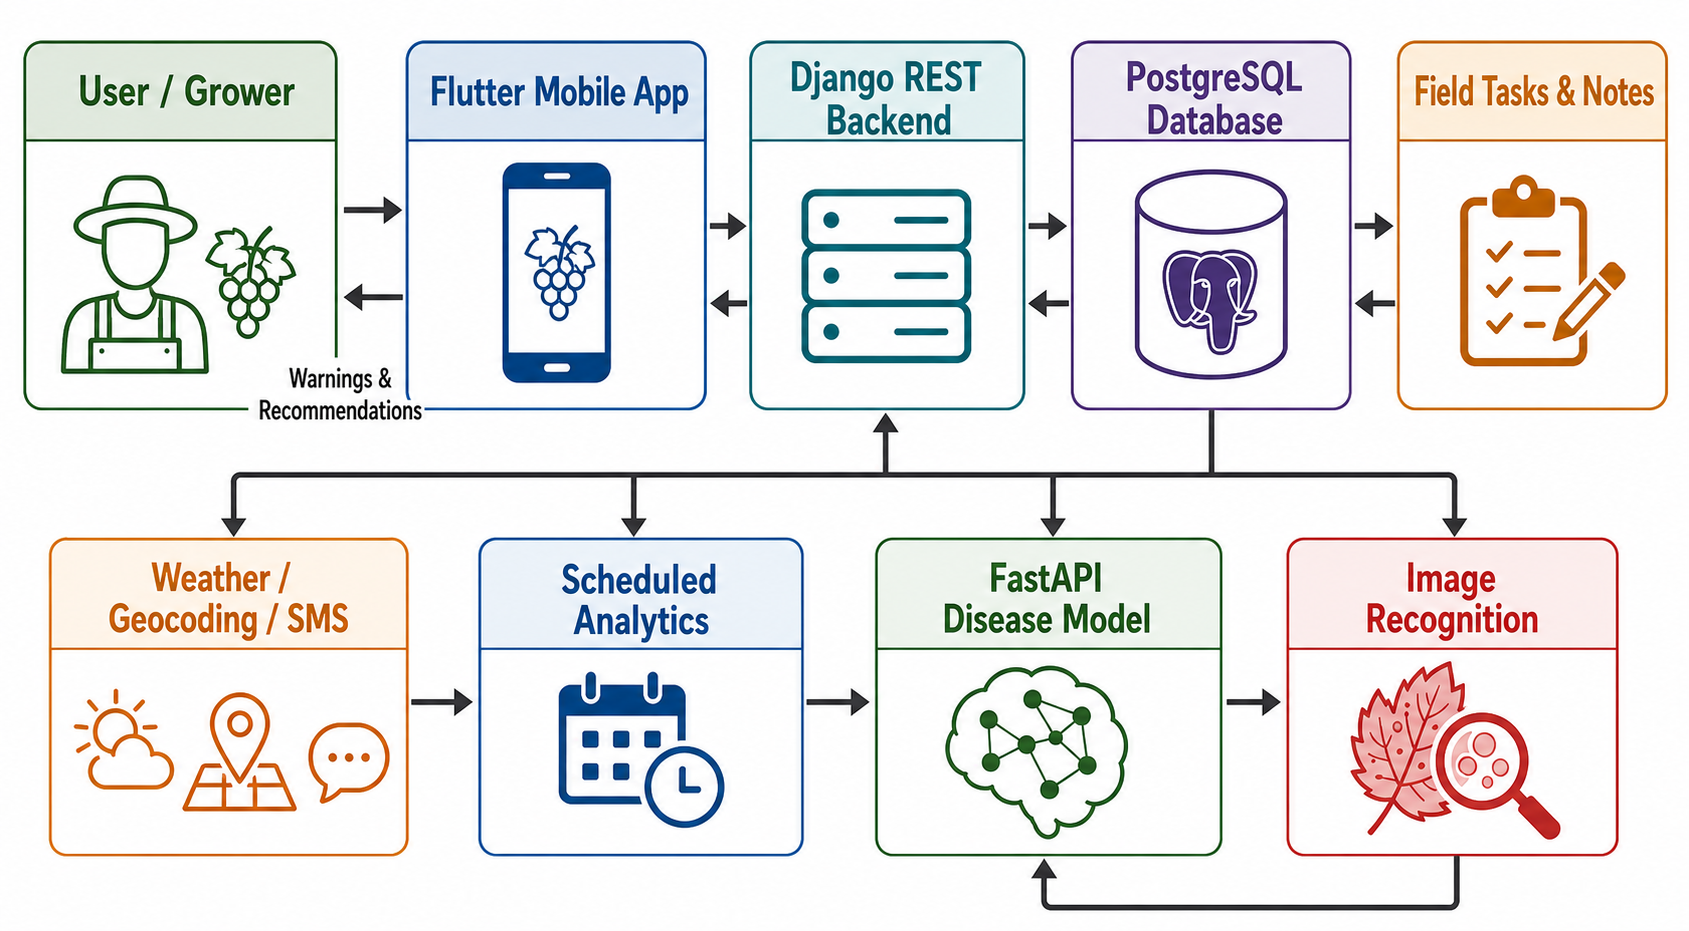
\includegraphics[width=\linewidth]{../fig/fig1_system_architecture_v2.png}
\caption{Conceptual architecture of the GrapeMaster platform. The platform connects mobile field operations, backend business services, relational storage, scheduled analytical workflows, disease-risk simulation, image-analysis modules, and external data services.}
\label{fig:conceptual_architecture}
\end{figure}

\subsection{Logical Architecture}

The logical architecture follows the same five-part structure used in the implementation section. Rather than treating the platform as a set of isolated modules, GrapeMaster organizes the application, data, analytical models, image diagnosis, and operational feedback as a connected decision-support workflow. Table~\ref{tab:architecture_layers} summarizes these layers, while Figure~\ref{fig:interaction_flow} illustrates how users, software services, data sources, and models interact.

\begin{table}[H]
\centering
\caption{Logical architecture layers of GrapeMaster.}
\label{tab:architecture_layers}
\small
\begin{tabular}{@{}p{0.21\linewidth} p{0.39\linewidth} p{0.34\linewidth}@{}}
\toprule
Layer & Main components & Main responsibilities \\
\midrule
Application and presentation layer & Dart/Flutter modules for fields, tasks, recognition, forum, maps, notes, authentication, weather, and notifications; Kotlin/Gradle and Java-compatible Android shell & Mobile interaction, field input, weather and warning display, task operation, image upload, and grower communication \\
Data ingestion and storage layer & Python, Django REST Framework, PostgreSQL, Django Channels, Django APScheduler, SimpleJWT, master-data modules & API routing, authentication, data persistence, scheduled data updates, WebSocket routing, and business records \\
Phenology and disease analytics layer & Python weather processing, Pandas, NumPy, GDD and Wang--Engel phenology model, spraying-suitability workflow, FastAPI disease-risk model & Weather transformation, growth-stage simulation, disease-risk simulation, treatment-window generation, and risk interpretation \\
Image-based diagnosis layer & Python, PyTorch, TorchVision, OpenCV, Pillow, Ultralytics YOLO/SAM, EfficientViT, UNet, segmentation, recognition and reporting modules & Disease-image upload, detection, recognition, segmentation, processed-image generation, and symptom-level evidence extraction \\
Task recommendation and alert layer & Notice services, task services, fungicide-history conversion, action recommendations, treatment windows & Warning delivery, task recommendation, plant-protection feedback, overdue handling, and recalculation after completed operations \\
\bottomrule
\end{tabular}
\end{table}

At the application and presentation layer, the Flutter mobile client provides the operational entry point for growers. It handles field creation, crop-season inspection, weather and warning display, image upload, plant-protection and irrigation tasks, field notes, disease reporting, and forum communication. This layer translates analytical results into field-level interaction rather than treating the system as a model-execution environment alone.

At the data ingestion and storage layer, the Django REST backend receives mobile inputs and coordinates persistence in PostgreSQL. Field boundaries, crop seasons, weather records, phenology outputs, disease-risk outputs, fungicide and pesticide master data, tasks, notes, notices, messages, and forum records are stored as linked business entities. The crop season is the main data anchor because it connects field geometry, cultivar information, weather, phenology, disease risk, operations, and observations.

At the phenology and disease analytics layer, scheduled backend workflows retrieve weather data, transform hourly and daily weather variables, simulate grapevine phenology, evaluate spraying suitability, and construct disease-model requests. The independent FastAPI disease-model service receives weather, growth stage, cultivar susceptibility, disease targets, and fungicide-history inputs, then returns infection risks, stress risks, field risks, protection times, action recommendations, and treatment windows.

At the image-based diagnosis layer, uploaded field images are processed by backend image-analysis modules. YOLO, ViT or EfficientViT, UNet, and segmentation-related components support disease detection, recognition, segmentation, processed-image generation, and severity-related outputs. This layer complements weather-driven disease-risk analytics by adding symptom-level evidence from field observations.

At the task recommendation and alert layer, analytical outputs are converted into user-facing decisions. Warnings, treatment windows, recommendations, spraying-suitability indicators, and overdue task states are delivered through notices and task interfaces. Completed plant-protection tasks are converted into fungicide-history records, which are then used in later disease-risk recalculation. This feedback mechanism closes the management loop from model output to field operation and back to model input.

Figure~\ref{fig:interaction_flow} describes the interaction among users, data sources, software layers, frontend interfaces, backend services, and analytical models.

\begin{figure}[htbp]
\centering
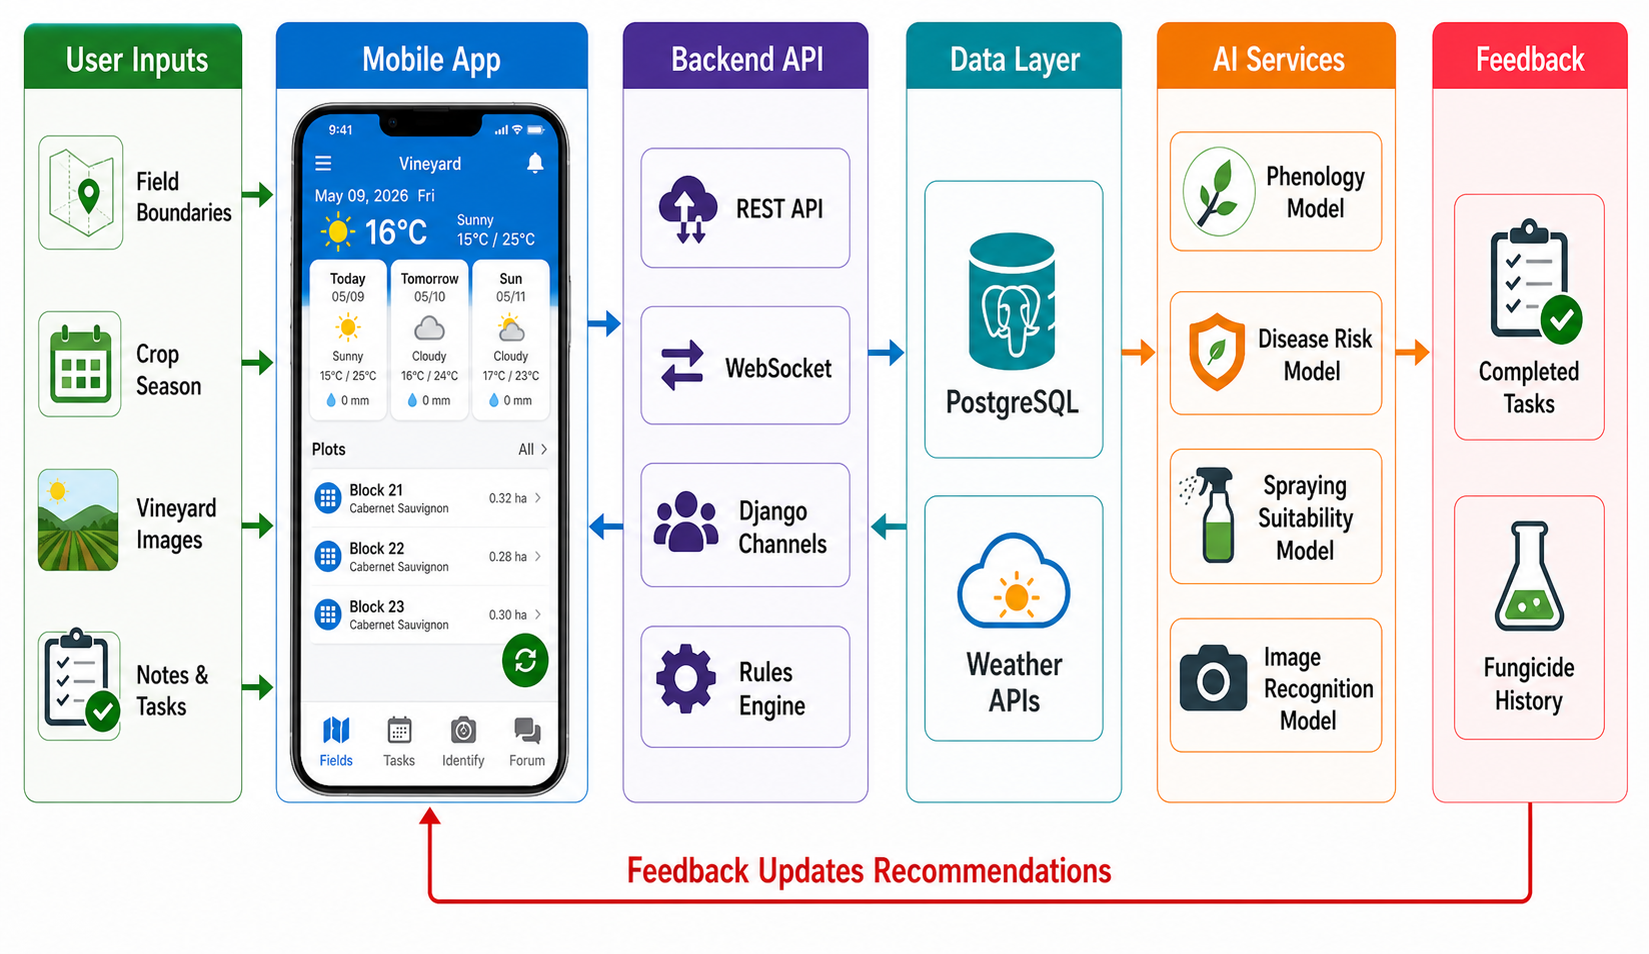
\includegraphics[width=\linewidth]{../fig/fig2_interaction_flow.png}
\caption{Interaction flow among users, mobile frontend, backend services, data sources, analytical models, and management feedback in GrapeMaster.}
\label{fig:interaction_flow}
\end{figure}

\section{Implementation}

\subsection{Application and Presentation Layer Implementation}

The application layer is implemented as a Flutter mobile client written in Dart. The Android project shell uses Kotlin and Gradle on the Java-compatible Android toolchain for platform integration, while the cross-platform user interface and business interaction logic remain in Flutter. Following the layered reporting style of end-to-end agricultural platforms, the client was designed as the operational entry point rather than only a visualization front end. The main navigation contains four modules: field management, task management, image-based recognition, and forum communication. The field module is the core workspace. It supports vineyard field creation and inspection, crop-season selection, weather display, growth-stage information, disease-risk review, notifications, field sharing, and recycle-bin operations. The task module supports plant-protection and irrigation workflows, including task creation, update, completion, deletion, and overdue-state handling. The recognition module supports image selection from camera or album, local image resizing and compression, image upload, disease recognition, severity inspection, disease reporting, historical diagnosis messages, and WebSocket-based intelligent-recognition interactions. The forum module supports grower communication through posts, comments, replies, and reply notifications.

The mobile client uses dio, http, and requests packages for REST requests, and web socket channel support for real-time interactions. Local state such as user credentials, selected fields, selected crop seasons, and user preferences is stored through shared preferences. Location and map functions are implemented with AMap packages, geolocator, geojson, and flutter map. Image-related workflows use image picker, the Dart image package, flutter image compression, and multipart upload. Weather, phenology, disease-risk, task, note, notification, and forum records are rendered through native Flutter pages, while charts and media-related displays use packages such as fl chart, carousel slider, flutter svg, webview flutter, flutter pdfview, and video player. In this implementation, the mobile interface converts analytical outputs into field-oriented interactions: a warning can lead to a plant-protection task, a completed task can update the disease-model fungicide history, and an image diagnosis can lead to disease reporting or consultation.

\subsection{Data Ingestion and Storage Implementation}

The backend is implemented in Python with Django 4.2 and Django REST Framework, with PostgreSQL as the main structured database. Database access uses \texttt{psycopg2} and the Django ORM, while configuration and environment variables are handled with \texttt{python-decouple}. The service exposes REST endpoints for users, fields, crop seasons, master data, weather, phenology, disease risk, tasks, notes, notices, messages, forums, model outputs, image processing, application updates, and feedback. SimpleJWT and PyJWT are used for token-based mobile authentication. Django Channels provides WebSocket routing for notice delivery and intelligent-recognition sessions, while Django APScheduler and APScheduler support scheduled weather and model workflows. API documentation and schema support are provided through DRF schema tools and \texttt{drf-yasg}. Cross-origin access is handled through \texttt{django-cors-headers}.

The data model is organized around two primary agricultural entities: the vineyard field and the crop season. The field record stores the user, field name, area, GeoJSON boundary, centroid longitude and latitude, administrative region, sharing state, deletion state, notice state, and a generated field-boundary preview. When a field is saved, the backend parses the GeoJSON boundary, derives a boundary image, estimates the field area, calculates the centroid, and requests geocoding information from an external service. Geospatial processing uses Python packages such as Shapely, Fiona, GeoPandas, Matplotlib, and Geopy, while external service calls use Requests or HTTPX. The crop-season record links the field with cultivar, cultivation method, vine age, field coordinates, field size, and cultivar metadata. This record is the main relational anchor for weather records, phenology outputs, disease-risk outputs, fungicide and irrigation tasks, notes, warnings, and user-facing summaries.

Master-data tables store grape varieties, cultivar susceptibility, fungicides, pesticides, BBCH growth stages, cultivation methods, disease types, and reminder rules. The fungicide table provides the parameters needed to transform task records into disease-model inputs. It stores target disease, preventive protection days, curative protection days, efficacy parameters, suitable growth-stage range, dose information, active ingredients, and safety information. This design allows the backend to convert user-completed plant-protection tasks into structured fungicide-history records rather than treating them only as calendar events.

The implementation stores both normalized relational records and JSON model payloads. Weather, phenology, disease-risk, and disease-request-body records can therefore be served to the mobile client while preserving the original model inputs and outputs needed for recalculation, auditing, and future validation. This hybrid pattern is useful for a decision-support platform because model workflows often require nested time-series data that do not fit naturally into a single relational table.

\subsection{Phenology and Disease Analytics Implementation}

\subsubsection{Weather Processing}

For each active crop season, scheduled Python backend jobs retrieve historical and forecast weather using the centroid of the vineyard field. The weather workflow uses HTTP clients such as Requests, HTTPX, \texttt{openmeteo\_requests}, \texttt{requests\_cache}, and \texttt{retry\_requests} to request historical data from the beginning of the current year to the previous day and combine these observations with a 16-day forecast. Hourly variables include air temperature, relative humidity, dew point, precipitation, wind speed, and wind gusts. Daily variables include maximum, minimum, and mean temperature, precipitation, maximum wind speed, maximum gust speed, sunrise time, and sunset time. Missing values are filled by carrying forward the previous available value before the records are used by analytical modules.

The backend converts these data into three working schemas using Pandas, NumPy, Python Dateutil, Pytz, and standard JSON processing. First, daily mean temperature is transformed into phenology-model input. Second, hourly weather is transformed into the disease-model schema, including datetime, dew point, precipitation, relative humidity, air temperature, and wind speed. Third, short-term hourly records are used to evaluate spraying suitability. This preprocessing stage coordinates different model requirements while maintaining a single crop-season data anchor.

\subsubsection{Phenology Simulation}

The phenology workflow is implemented in Python and estimates grapevine growth-stage progression from daily mean temperature and crop-season metadata. The implementation uses Pandas and NumPy to calculate a Wang--Engel temperature response function and daily growing degree days (GDD). Daily GDD values are accumulated into \texttt{GDDCUSUM}. The accumulated heat is then mapped to BBCH principal stages using region-, cultivar-, or maturity-specific thresholds stored in the model parameter file. The output contains date, GDD, accumulated GDD, BBCH principal stage, and one-digit BBCH class. The backend joins these outputs with BBCH master data to add growth-stage codes and Chinese and English descriptions for mobile display.

The phenology output has two functions in the platform. It provides growers with a crop-development timeline and supplies the disease-risk model with a daily growth-stage sequence. This connection is essential because grapevine disease relevance and risk interpretation depend on susceptible phenological windows as well as weather conditions.

\subsubsection{Disease-Risk Simulation}

Disease-risk simulation is provided by an independent Python FastAPI service with a \texttt{/simulate} endpoint. The service uses Uvicorn for ASGI serving and Pydantic models for request validation and typed schema definition. The Django backend constructs a crop-season-level request body containing crop-season identifiers, region, crop EPPO code, latitude, longitude, request date, hourly weather, growth-stage sequence, historical fungicide applications, target disease codes, cultivar susceptibility values, requested features, and date ranges. In the current vineyard workflow, the main target disease codes are \texttt{PLASVI} for grape downy mildew and \texttt{UNCINE} for grape powdery mildew. The model service also contains additional grape disease modules, but the operational backend workflow primarily consumes downy mildew and powdery mildew outputs.

Inside the disease-model service, the request body is parsed into a crop-season object. The service dynamically loads the crop implementation according to the crop EPPO code and dynamically initializes the requested disease modules. Numerical and tabular computation is performed mainly with Pandas and NumPy, while date handling uses Python Dateutil and Pytz. The grape disease implementation calculates daily weather favorability from hourly weather. For infection favorability, the model uses temperature response, relative-humidity-derived wetness duration, and disease-specific thresholds. It then applies growth-stage correction, cultivar susceptibility correction, and fungicide-effect correction. Daily favorability values are classified into infection-risk categories, and a rolling short-term aggregation is used to derive more stable disease-risk states.

The disease-risk workflow also includes disease-onset logic. It estimates primary inoculum availability, inoculum maturation, spore release, and potential infection events using weather and disease parameters. Dates before modeled disease onset are downgraded to unfavorable states, and dates outside the configured BBCH disease window are treated as non-seasonal. Fungicide records can convert otherwise risky days into protected days when preventive or curative protection effects are active.

The model returns daily infection risks, stress risks, field risks, stress protection times, action recommendations, and treatment windows. Field risk is derived from the individual disease risks by selecting the highest relevant unprotected risk while preserving fully protected states when all target diseases are protected. The backend compresses these outputs into date-aligned arrays and stores them in the disease-data table for mobile display and later use.

\subsubsection{Spraying Suitability Assessment}

The spraying-suitability workflow evaluates whether short-term weather conditions support plant-protection operations. The implementation considers air temperature, current precipitation, wind speed, relative humidity, precipitation expected in the next hours, cultivation method, sunrise time, and sunset time. The resulting suitability indicators are calculated for the forecast horizon and stored with crop-weather records. These indicators allow the system to connect disease-risk warnings with practical execution conditions, reducing the chance that a recommended treatment is scheduled under unsuitable weather.

\subsubsection{Model-Guided Input Optimization}

The disease-risk and spraying-suitability workflows jointly provide the analytical basis for model-guided plant-protection input optimization. As summarized in Figure~\ref{fig:input_optimization}, GrapeMaster integrates weather records, cultivar information, soil and field data, and agrochemical master data within a crop-season analytical workflow. This integration allows recommendations to be expressed not only as disease-risk warnings, but also as operational decisions concerning input selection, application timing, spray frequency, and dose optimization.

\begin{figure}[htbp]
\centering
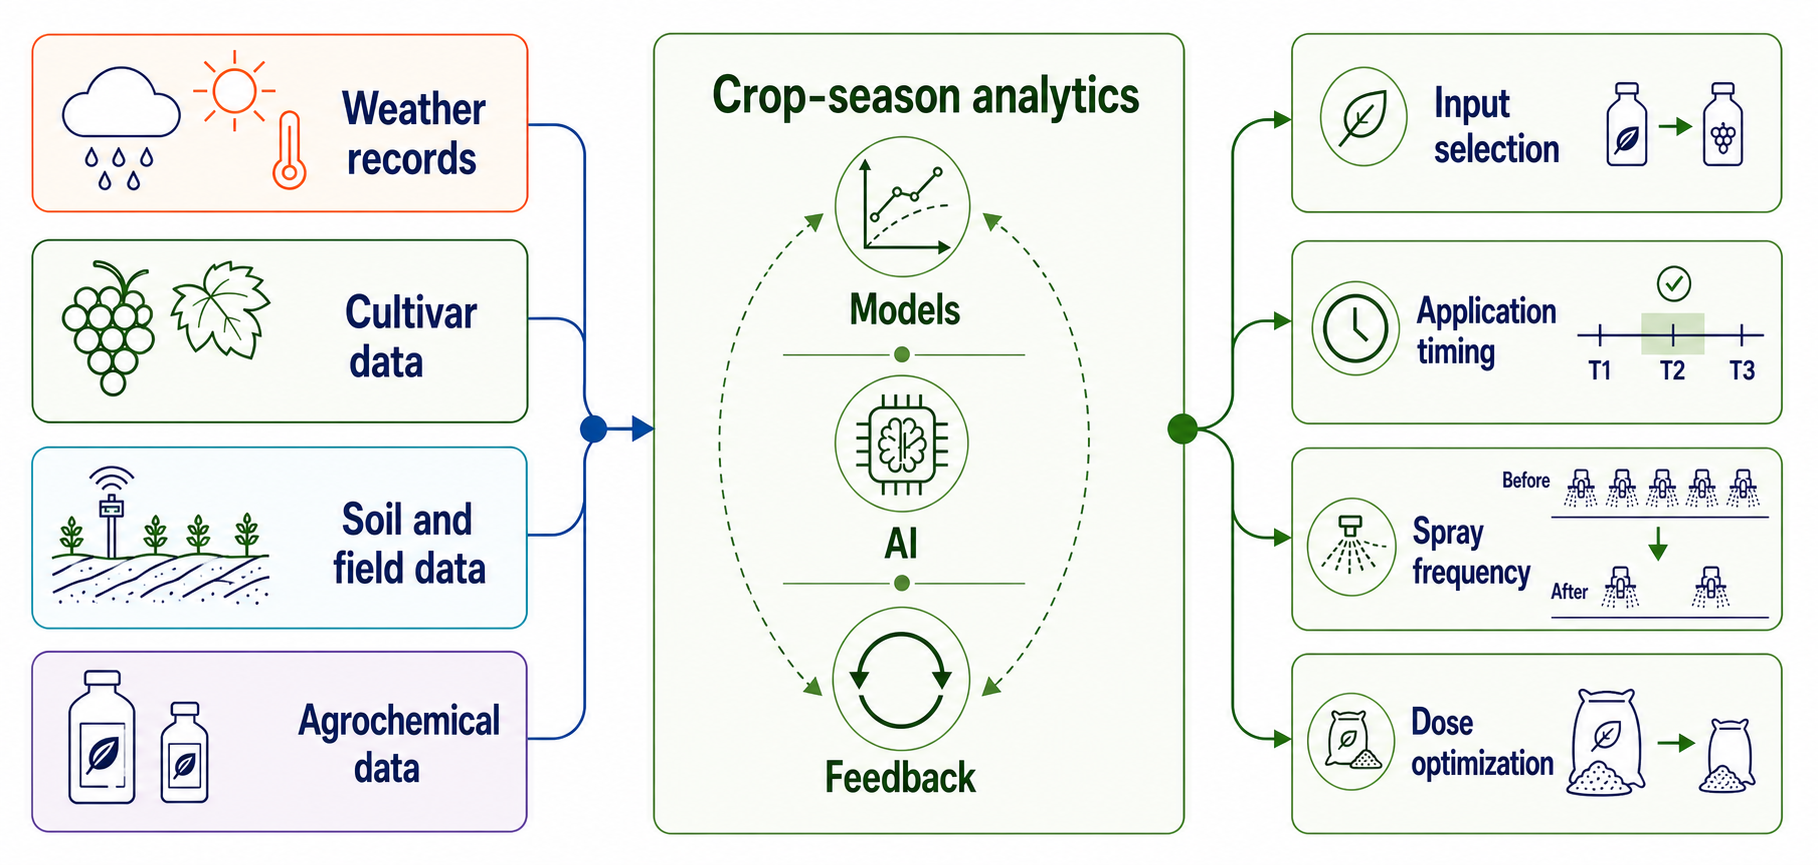
\includegraphics[width=\linewidth]{../fig/fig3_input_optimization.png}
\caption{Model-guided optimization of vineyard plant-protection inputs in GrapeMaster. Weather records, cultivar data, soil and field information, and agrochemical master data are integrated within the crop-season analytical workflow to support input selection, application timing, spray-frequency reduction, and dose optimization.}
\label{fig:input_optimization}
\end{figure}

\subsection{Image-Based Diagnosis Implementation}

The image-based diagnosis layer is implemented in Python as a set of backend image-processing endpoints and model modules. The mobile client uploads images through multipart requests after local selection and preprocessing. For disease classification, the backend uses PyTorch and an EfficientViT-based classifier that maps uploaded grape images to disease or healthy categories and returns corresponding prevention or management text. Pillow is used for image loading in the classifier workflow, while model execution uses PyTorch tensors and EfficientViT model-zoo utilities. The current category mapping includes grape leaf blight, grape black rot, grape Esca or black measles, healthy grape, and grapevine yellowing.

The platform also includes a segmentation-based severity pipeline. The pipeline uses OpenCV, NumPy, PyTorch, TorchVision transforms, and Ultralytics model components. It first applies YOLO to locate leaf or leaf-disc regions, then uses MobileSAM to segment the leaf region from the detected box, and finally applies a UNet model to segment lesion and leaf pixels in the cropped region. Severity is calculated as the percentage of lesion pixels relative to the sum of lesion and leaf pixels:

\begin{equation}
\label{eq:severity}
\mathrm{Severity} = \frac{N_{\mathrm{lesion}}}{N_{\mathrm{lesion}} + N_{\mathrm{leaf}}} \times 100.
\end{equation}

The output includes a processed image with bounding boxes and severity labels, together with per-region severity values. This image pathway complements weather-driven disease-risk analytics by adding symptom-level evidence from field observations. It also provides a route for users to report observed disease events, which can support future validation of model warnings.

\subsection{Task Recommendation and Alert Implementation}

Task recommendation and alert functions connect analytical outputs with field operations. Disease-risk outputs, phenology changes, treatment windows, spraying-suitability indicators, field-sharing events, and task states are stored by the backend and exposed to the mobile application through warning, notification, and task interfaces. The notice service stores title, message text, importance, read state, user, and crop season. WebSocket channels are used to deliver timely notice updates to the mobile client. Users can mark notices as read, accept shared fields, inspect crop-season warnings, and create plant-protection or irrigation tasks from warning contexts.

Plant-protection and irrigation tasks are implemented as persistent business objects. Each task stores crop season, execution date, task type, task status, field name, and task-specific parameters. If a task remains unexecuted after its execution date, the backend marks it as overdue. For plant-protection tasks, linked fungicide records store product name, dose, dose unit, and total unit. When a user creates, updates, deletes, or completes a plant-protection task, the backend compares the fungicide list and execution date with the previous record and updates the disease-model fungicide history when needed.

Completed plant-protection tasks are converted into applied-fungicide inputs for subsequent disease-risk recalculation. The backend derives application date, target disease, preventive protection period, curative protection period, and efficacy-related parameters from the task record and fungicide master data. This produces a feedback loop in which a field operation changes the future disease-risk trajectory. Thus, GrapeMaster records whether recommended actions were completed and incorporates completed operations into later risk simulation.

\section{Deployment}

GrapeMaster was deployed in multiple viticultural regions in China, including Yangling in Shaanxi Province, Nanning, Du'an of Hechi, and Xing'an of Guilin in Guangxi Province. These sites represent different climatic and management settings and provide an initial basis for examining whether the platform can support disease warning and spray-timing decisions beyond a single vineyard context. Figure~\ref{fig:trial_distribution} shows the geographic distribution of the deployment sites. During deployment, the platform was used for spore monitoring, disease warning, and plant-protection scheduling. Field observations indicated that initial spore capture preceded the first visible disease symptoms by approximately one to two months, and that the first major spore peak broadly coincided with the period of rapid disease development. These observations suggest that the platform can provide a warning signal earlier than symptom-based scouting while retaining temporal consistency with subsequent epidemic acceleration.

\begin{figure}[htbp]
\centering
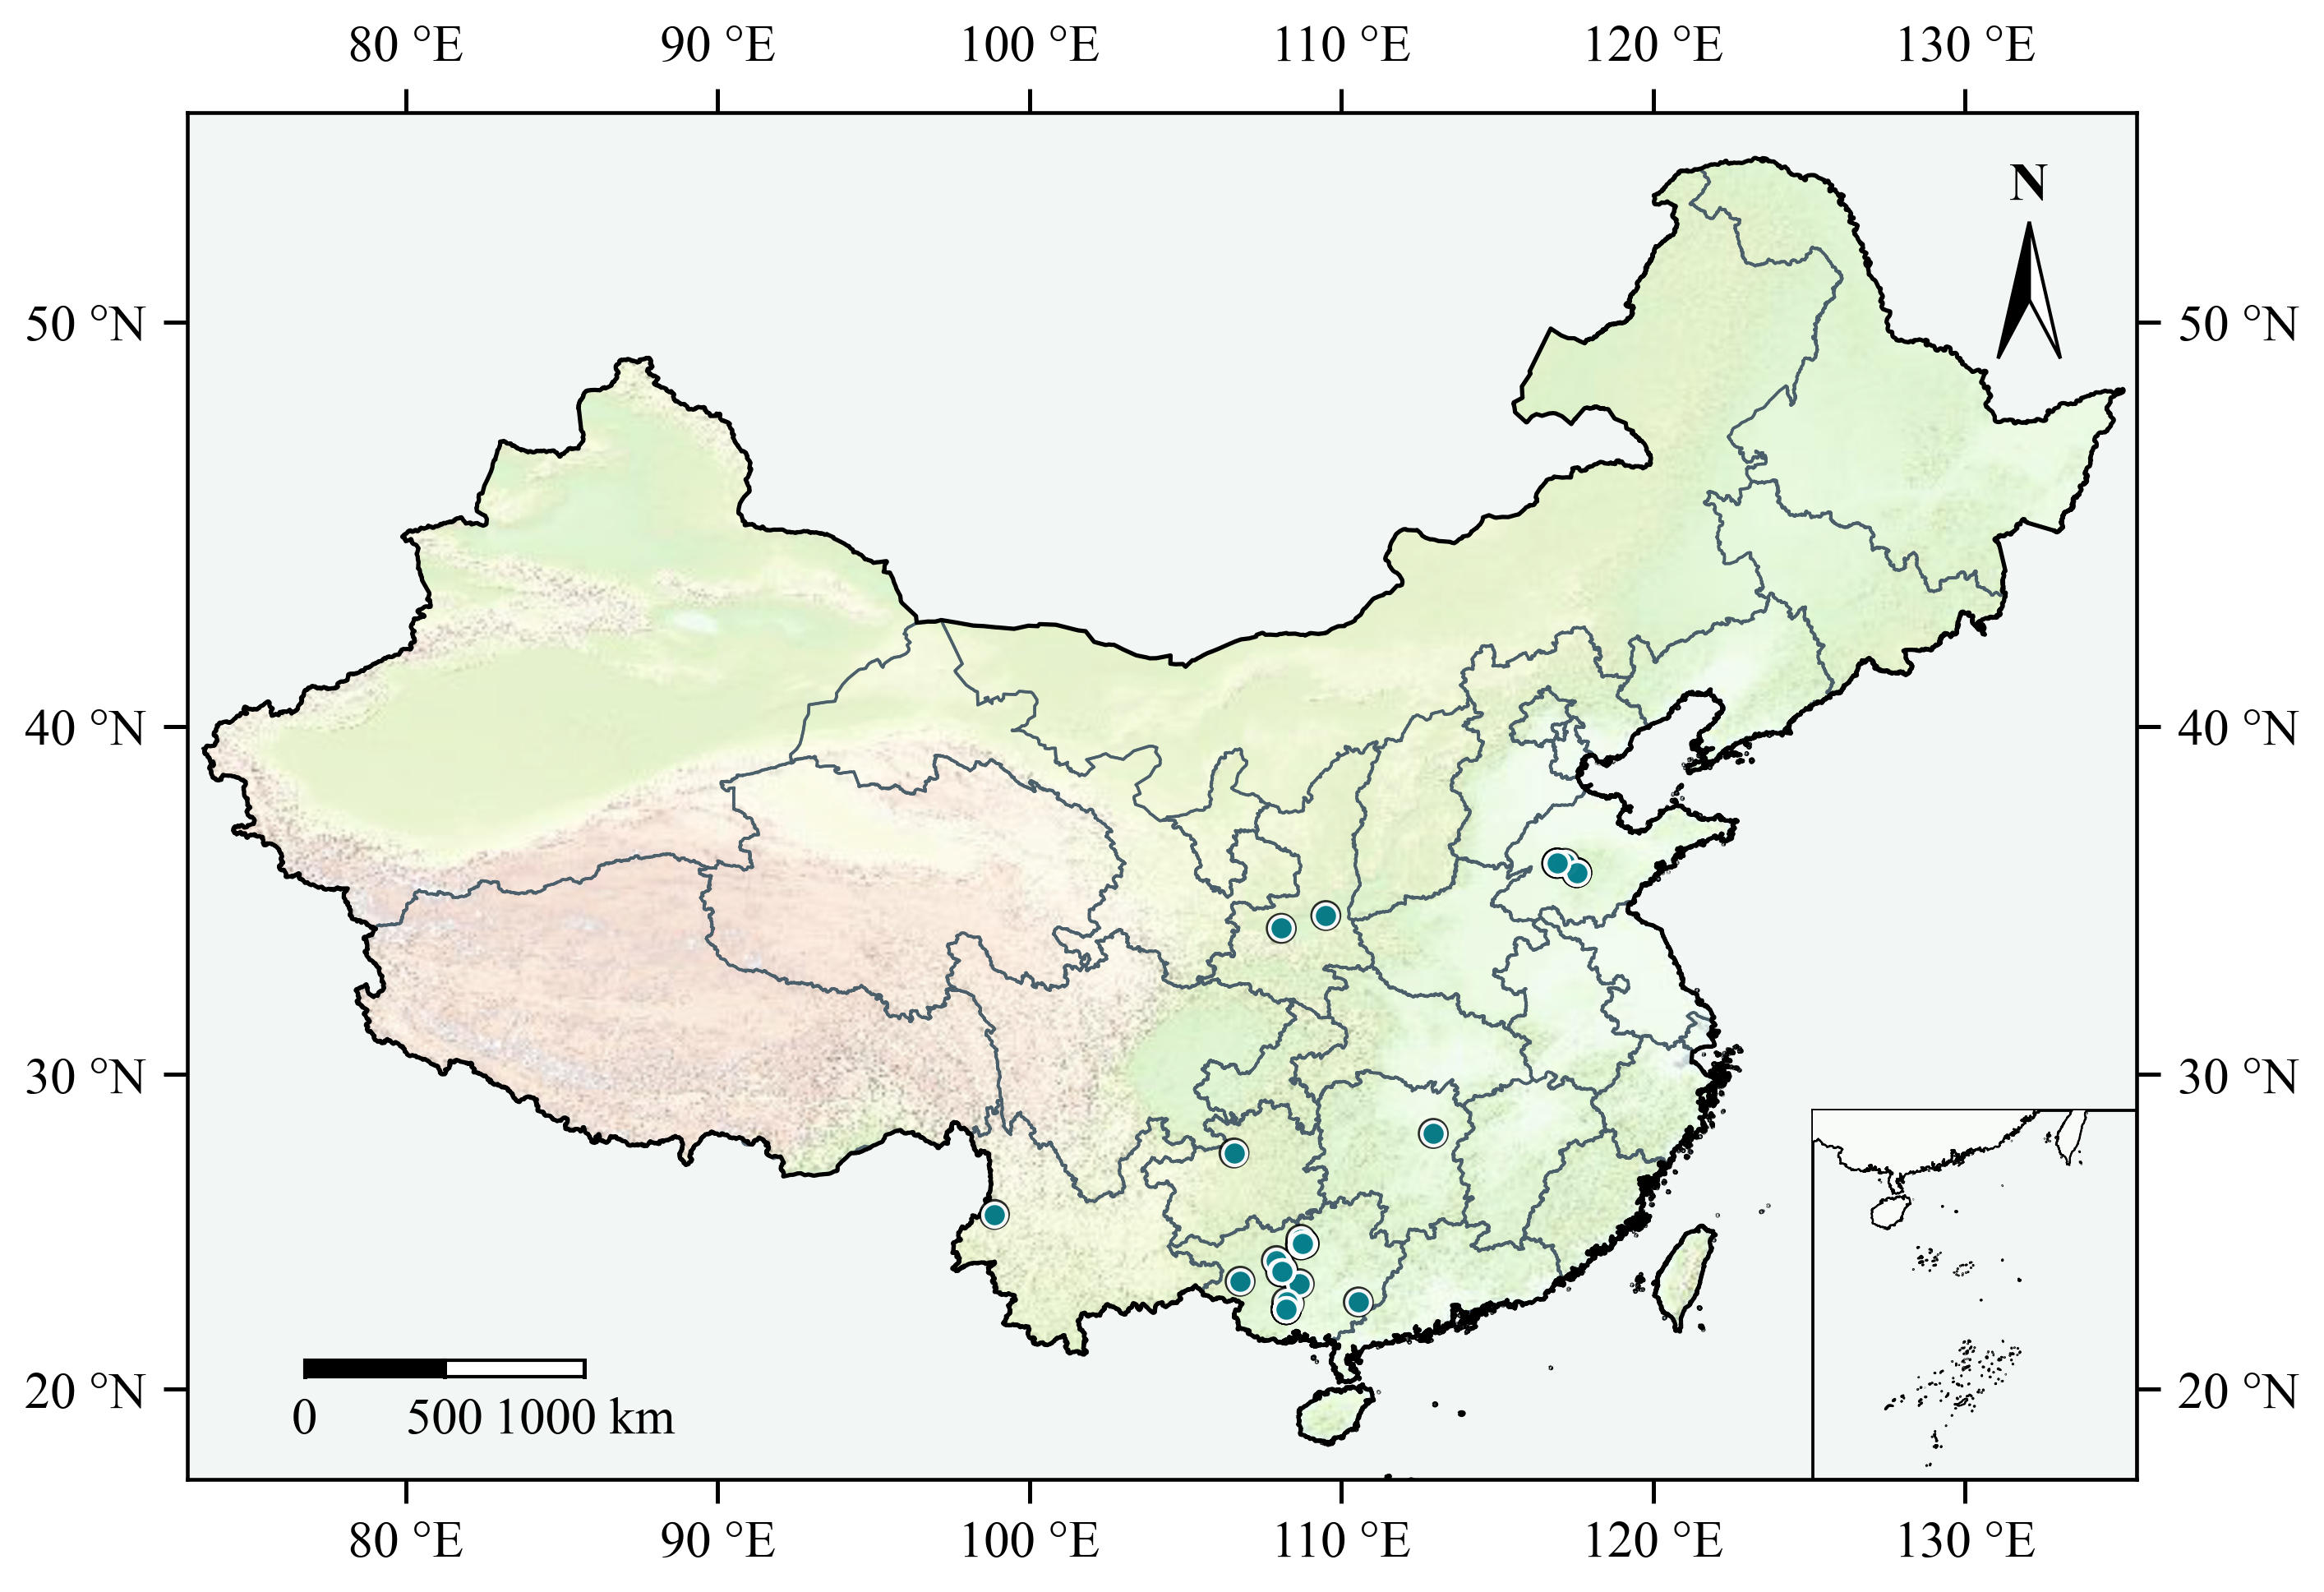
\includegraphics[width=\linewidth]{../fig/grape_trial_distribution_china.png}
\caption{Geographic distribution of GrapeMaster deployment sites in China. The mapped sites include Yangling in Shaanxi Province and Nanning, Du'an, and Xing'an in Guangxi Province.}
\label{fig:trial_distribution}
\end{figure}

Operational comparisons with routine grower practice further indicated that model-guided timing could reduce fungicide applications by at least three sprays per season. To express this result as a management benefit, direct costs were estimated for fungicide inputs, spraying equipment, and labor in a representative spray program used in the deployment regions. Under this cost structure, each avoided fungicide spray saved approximately 384.75 CNY ha$^{-1}$, and a three-spray reduction saved approximately 1154 CNY ha$^{-1}$ yr$^{-1}$. Extrapolated to different vineyard scales, the estimated annual savings were 1.154$\times10^{4}$ CNY for 10 ha, 1.154$\times10^{5}$ CNY for 100 ha, and 1.154$\times10^{6}$ CNY for 1000 ha.

Taken together, the deployment results show technical operability across multiple grape-growing regions and provide preliminary evidence that the platform can support earlier warning and reduced fungicide use. Under the cost structure used here, each avoided spray saved approximately 384.75 CNY ha$^{-1}$, and a three-spray reduction saved approximately 1154 CNY ha$^{-1}$ yr$^{-1}$. These reductions decrease pesticide, equipment, and labor costs while supporting lower-input disease management. Table~\ref{tab:deployment_benefit} summarizes these deployment-related economic estimates.

\begin{table}[H]
\centering
\caption{Estimated economic benefit of reducing three fungicide sprays under the deployed GrapeMaster workflow.}
\label{tab:deployment_benefit}
\begin{tabular}{p{0.22\linewidth} p{0.22\linewidth} p{0.36\linewidth}}
\toprule
Vineyard type & Typical scale & Estimated annual saving \\
\midrule
Small vineyard & 10 ha & 11{,}540 CNY yr$^{-1}$ \\
Medium vineyard & 100 ha & 115{,}400 CNY yr$^{-1}$ \\
Large vineyard & 1000 ha & 1{,}154{,}000 CNY yr$^{-1}$ \\
\bottomrule
\end{tabular}
\end{table}

\section{Features and Functionalities}

GrapeMaster provides user-facing functions through four principal mobile workspaces: vineyard field management, task management, intelligent recognition, and grower communication. These workspaces share a crop-season context, allowing weather information, phenological status, disease warnings, image evidence, field notes, and completed operations to be displayed and updated for the same vineyard season.

\subsection{Vineyard Field and Crop-Season Management}

The field-management function provides the spatial entry point of the platform. Users can create, inspect, edit, share, delete, recover, and select vineyard fields. During field creation, the mobile client supports map-assisted input and records the field name, boundary geometry, area, centroid longitude and latitude, administrative region, and a generated boundary preview. Each field is displayed as a selectable field card in the mobile workspace, from which users can access crop seasons, weather, warnings, notes, tasks, and field settings.

The platform treats field sharing as a managed collaboration function rather than only a data export operation. A user can invite another account to access a field. The recipient receives a field-sharing notice, accepts the invitation from the notification interface, and then sees the shared field in the operational field list. Deleted fields are moved into a recycle-bin workflow so that accidental deletion does not immediately remove the field from user interaction. This supports practical field management in situations where vineyards are operated by multiple users or where historical field information must remain recoverable.

The crop-season function links a vineyard field with grape variety, cultivation method, vine age, field area, and coordinates. It is the central working unit of the platform: weather retrieval, phenology simulation, disease-risk calculation, plant-protection tasks, irrigation tasks, notes, and alerts are all associated with a crop season. This design is appropriate for perennial crop management because the same vineyard field persists across production years, whereas each season requires separate weather records, growth-stage trajectories, disease-risk outputs, and field-operation histories.

Within the crop-season workspace, users can view the selected cultivar and cultivation method, inspect the current growth-stage context, open disease-warning information, review weather details, and enter task or note pages without manually reselecting the field. The workspace therefore makes the crop season the operational decision context and keeps weather, disease, notes, and tasks attached to the same field-season object.

\subsection{Weather, Phenology, and Spraying-Suitability Display}

The weather function provides field- and crop-season-specific environmental information. The backend retrieves and stores hourly and daily weather variables according to the field centroid, while the mobile client presents these data as near-term weather summaries, hourly weather records, and multi-day forecast views. Hourly displays include temperature, relative humidity, precipitation, and wind speed. Daily displays include precipitation, maximum and minimum temperature, mean temperature, maximum wind speed, gust-related indicators, and weather-status information. These views allow users to inspect the local environmental conditions that explain disease warnings and task feasibility.

The phenology function displays predicted grapevine growth stages for the selected crop season. The backend calculates daily GDD, accumulated GDD, BBCH principal stages, one-digit BBCH stages, and growth-stage descriptions, and the mobile client presents the resulting stage information to users. The displayed growth-stage information has two direct management roles. First, it gives users a seasonal development reference when inspecting the field. Second, it explains why disease warnings or plant-protection recommendations may become more or less relevant as the crop enters susceptible growth stages.

The spraying-suitability function converts short-term weather conditions into field-operation guidance. It considers temperature, precipitation, wind speed, relative humidity, near-future rainfall, cultivation method, sunrise, and sunset. The mobile client can therefore display both disease pressure and near-term spraying feasibility. This function is relevant when a treatment window is open but rainfall, wind, or unsuitable timing may reduce spray effectiveness or prevent safe execution.

\subsection{Disease-Risk Warning and Treatment-Window Review}

The disease-warning function presents model-derived disease-risk information for the selected crop season. The backend stores date-aligned disease-risk outputs for target grape diseases, including downy mildew and powdery mildew in the main operational workflow. The mobile client retrieves and displays disease-risk summaries, infection-risk codes, stress-risk codes, field-risk codes, action recommendations, and treatment windows. The purpose of this function is to make daily model outputs readable as management information rather than as raw numerical arrays.

The warning display separates several kinds of information that growers need to interpret together. Infection risk describes whether weather and disease conditions are favorable for infection. Stress risk summarizes disease-related pressure under recent or short-term conditions. Field risk integrates the disease-specific results into a crop-season-level warning state. Protection-related states indicate whether previous fungicide applications are still considered active by the model. Action recommendations translate these states into practical guidance, including whether treatment is recommended, delayed, or regarded as unnecessary because protection is already active.

The treatment-window function translates model risk into management timing. A future window indicates that a recommendation is approaching, a current window indicates that the recommended treatment period is active, and a missed window indicates that the suggested timing has passed while the risk remains relevant. This design reduces the need for users to infer timing from weather, phenology, and risk codes, and provides a direct bridge from disease warning to task creation.

The warning function is connected with notifications. When phenology changes or disease-risk states trigger an alert, the backend generates user-specific notices. These notices can be reviewed, marked as read, or used as entry points for related operations such as task creation. In this way, disease-risk information is exposed through both the field workspace and the notification workflow, which supports users who do not continuously inspect each field page.

\subsection{Plant-Protection and Irrigation Task Management}

The task module supports two major operation types: plant protection and irrigation. Users can create, inspect, edit, complete, and delete tasks. Each task is associated with a crop season and contains execution time, field name, task status, and operation-specific parameters. The task list allows users to inspect planned, completed, and overdue operations for the selected crop season or user account. Tasks that remain unexecuted after their scheduled execution date can be marked as overdue by the backend, allowing the interface to distinguish missed operations from pending ones.

Plant-protection tasks include container type, sprayer or mixer capacity, water consumption, execution date, task status, and one or more fungicide or pesticide records. The mobile task-creation workflow supports both large-container and sprayer-based mixing modes. Fungicide and pesticide records include product name, dose, dose unit, and total unit, allowing the task to represent the practical spray mixture rather than only a generic operation name. Users can revise task parameters before execution and mark tasks as completed after the field operation is carried out.

Once a plant-protection task is completed, the backend converts the operation into applied-fungicide history for the disease model. The completed task supplies the application date, target disease, and protection parameters derived from fungicide master data. This distinguishes GrapeMaster from a task calendar: completed operations are archived and also change the disease-risk model state by adding protection effects. Subsequent disease-risk recalculation can therefore reflect whether users acted on previous recommendations.

Irrigation tasks include irrigation method, growth-stage period, irrigation duration, irrigation dosage, execution time, and task status. This allows users to manage water-related operations in the same operational environment as plant protection, keeping crop-season activities organized around the same field and crop context.

\subsection{Image-Based Disease Assistance and Severity Estimation}

The recognition module supports field-image-based assistance. Users can select an image from the camera or gallery, preview it in the mobile client, and upload it for recognition. Before upload, the image can be resized and compressed to reduce transmission load. The backend image-recognition service classifies grape images into disease or healthy categories and returns corresponding diagnostic or management text to the user. The current recognition output includes grape leaf blight, grape black rot, grape Esca or black measles, healthy grape, and grapevine yellowing categories.

The severity-estimation function provides lesion-level analysis for disease images. The backend applies a detection-segmentation pipeline to identify leaf regions, segment leaf and lesion areas, generate a processed image, and calculate a severity percentage for each detected region. The mobile interface displays the processed image and severity information, allowing users to inspect both the recognition result and the visual evidence supporting it. This output converts qualitative symptom observation into a quantitative estimate of disease severity.

The recognition workflow is designed as a complement to model-based disease warning. Weather-driven models provide risk forecasts even before visible symptoms are present, while field images provide symptom-level evidence once disease signs are observed. The platform keeps these functions in the same mobile environment, allowing users to compare warning information, field symptoms, and their own notes without switching to a separate diagnostic tool.

\subsection{Field Notes, Growth-Stage Notes, and Disease Records}

The note module supports user-entered field records. Users can create ordinary crop notes, growth-stage notes, and disease-incidence notes. These records can include text, date, crop-season context, disease or growth-stage selections, and images. Notes provide a lightweight field diary for management events and observations that are not necessarily formal tasks, such as canopy observations, visible symptoms, abnormal weather effects, or informal inspection results.

Growth-stage notes allow users to record observed crop development and compare field observations with model-predicted growth stages. Disease notes record disease type, incidence-related information, and supporting images. These records support later interpretation of model results and future validation by linking model-predicted risk periods with user-observed field symptoms. At the system level, the note function creates structured field evidence that can be connected with disease warnings and image-recognition records.

\subsection{Disease Reporting and Warning Feedback}

The reporting function allows users to submit observed disease events from the field. Reports can include user identity, field context, disease information, geographic information, and images. The backend can convert such reports into warning records and notify relevant users. This function gives the system an observation channel in addition to weather-driven simulation and image classification.

Disease reporting supports two-way information flow. The system sends warnings to users, while users can submit field evidence back to the system. This provides a basis for later model validation, regional warning refinement, and expert review. It also allows the platform to distinguish between simulated risk and user-confirmed disease occurrence when evaluating whether warnings correspond to field observations.

\subsection{Notifications, Field Sharing, and User Interaction}

The notification function provides user-specific alerts for disease warnings, task-related reminders, phenology-related operations, and field-sharing events. Notifications contain title, text, creation time, read state, importance, user, and crop-season association. The mobile client supports notification review, single-notice reading, grouped reading, important-notice review, and all-read operations. Some notifications provide direct actions, such as accepting a shared field or creating a task from a warning.

Real-time notification delivery is supported through WebSocket channels. This reduces the delay between backend event generation and user awareness, which is important for time-sensitive plant-protection recommendations. Notification settings can also be stored locally in the mobile client so that users can control how reminders are presented.

The platform also includes grower communication functions through the forum module. Users can create posts, upload images, inspect post details, add comments, reply to comments, and review reply notifications. This function supports practical information exchange among users, especially for field observations, disease symptoms, operation experience, and management questions that may not be fully captured by model outputs.

\subsection{User Account, Localization, and Auxiliary Services}

The user-account function supports login, profile information, local credential storage, and user-specific access to fields, tasks, notices, messages, and reports. Authentication allows the backend to associate operational records with specific users and to control access to field information. Local storage in the mobile client keeps selected user and field context available across sessions, reducing repeated input during field use.

The mobile application includes Chinese and English localization resources. Auxiliary services include suggestion and feedback submission, historical message review, PDF or document access, and application update support. These functions are not the core analytical contribution of the platform, but they support maintenance, communication, documentation, and user feedback within the mobile decision-support environment.

\section{Discussion}

The literature on vineyard disease management and agricultural decision support shows that effective decision support depends on the integration of predictive algorithms, monitoring, model outputs, management timing, and user interaction in a form that growers can act on \citep{McCown2002DSSComplexity,Rose2016DecisionSupportTools,Rossi2014ViteNet,Walling2020EDSS}. Recent work on farm management information systems, digital agriculture architectures, and viticulture decision support has further emphasized that system value emerges from the integration of data management, analytics, interfaces, and business processes rather than from isolated software functions alone \citep{Fountas2015FMIS,Tummers2019FMISReview,Tummers2021ReferenceArchitecture,Uyar2024DataValue,Knowling2021ViticultureModels}. GrapeMaster is therefore best interpreted as an integrated mobile software environment for crop-season management rather than as a standalone disease-warning model. The platform combines weather retrieval, phenology simulation, disease-risk modeling, image-based disease assistance, task execution, and notification delivery within one operational workflow. This system-level integration addresses the fragmentation problem in agricultural DSS deployment, where analytical functions, records, and management actions are often distributed across separate tools and lose decision value at the point of use \citep{McCown2002DSSComplexity,Fountas2015FMIS,Tummers2021ReferenceArchitecture,Walling2020EDSS}. By representing warnings, treatment windows, field observations, and operations within the same crop-season context, the architecture shifts the platform from model reporting toward operational decision support.

\subsection{System Integration}

The platform organizes analytical and operational data around the crop season rather than around a single model run or an isolated field record. This design matches the biological and managerial structure of vineyard disease control, in which risk depends on field location, cultivar susceptibility, phenological stage, recent weather, and prior treatment history \citep{Peng2024DownyMildew,Kunova2021PowderyMildew,Puelles2024DownyMildewModels}. By making the crop season the central unit, GrapeMaster connects field geometry, weather updates, BBCH-linked phenology outputs, disease warnings, fungicide applications, irrigation tasks, notes, and notices without requiring users to reconstruct context across separate modules. In software terms, this is consistent with the reference-architecture view that FMISs should integrate data management, operational records, and decision support within one coherent application structure \citep{Tummers2021ReferenceArchitecture}, and with viticulture modeling work that frames useful decision support as linking data streams to seasonal decisions rather than storing them in parallel silos \citep{Knowling2021ViticultureModels}.

The crop-season-centered design also gives the platform a temporal structure that is often absent from generic recording systems. Phenology is used to interpret disease relevance, fungicide applications are converted into model inputs that affect later risk states, and short-term weather is transformed into spraying-suitability assessments and treatment-timing cues. In this sense, the platform follows a principle emphasized in vineyard DSS research and integrated pest-management typologies: disease support is most useful when weather, crop development, and intervention timing are interpreted jointly \citep{Orlandini1993PLASMO,Rossi2014ViteNet,Marinko2024IPMTypology,Helps2024DSSValue,Knowling2021ViticultureModels}.

This organization is particularly relevant for vineyards because the same field persists across years, whereas the disease-relevant state of the crop changes continuously within a season. A field-only or disease-only data model is therefore too narrow. The crop season provides an intermediate unit that is stable enough for operational management while remaining specific to annual weather, phenology, and protection history. This design supports traceability from field creation to warning generation, task execution, and later management review.

\subsection{Operational Value}

The operational value of the platform lies in its combination of forecast-oriented and observation-oriented evidence. Weather-driven disease models have long been used to support fungicide timing, whereas recent computer-vision studies and sensing reviews have shown that image classification, detection, lesion segmentation, and proximal sensing can support disease recognition and severity estimation in grape production \citep{Puelles2024DownyMildewModels,Kunduracioglu2024GrapeDeepLearning,Shi2023SeverityAssessment,Liu2024FusionTransformerYOLO,Portela2024GrapevineSensingReview}. GrapeMaster brings these two evidence streams into the same mobile environment. Model outputs support warning before visible symptoms become severe, whereas uploaded field images, disease notes, and disease reports provide symptom-level evidence once disease can be observed directly. This combination is valuable because visual symptoms alone do not provide treatment timing or protection-state interpretation, while weather-driven risk values alone do not document whether symptoms are present or how severe they appear in the field \citep{Rossi2014ViteNet,Shi2023SeverityAssessment,Puelles2024DownyMildewModels,Portela2024GrapevineSensingReview}.

The platform also translates analytics into management actions. Many agricultural DSSs produce outputs that are scientifically meaningful but operationally indirect, such as risk indices, infection events, or model states that require interpretation before they can guide field activity \citep{Helps2024DSSValue,Walling2020EDSS}. In GrapeMaster, this translation is implemented through treatment windows, recommendations, spray-suitability indicators, and task objects. The task object gives the warning system a concrete operational endpoint: predicted risk can become a scheduled operation, and a completed operation can revise disease protection status.

The platform is not restricted to plant protection. The same crop-season workspace can include irrigation tasks, which is relevant in vineyard management because disease, canopy condition, water status, and seasonal crop development interact in practice even when they are modelled separately \citep{Kang2023IrrigationDSS,OrtegaFarias2019Phenology,Knowling2021ViticultureModels}. Although the present manuscript focuses on disease warning, the inclusion of irrigation functions shows how the platform can be extended into a broader viticultural management environment. This wider operational scope is aligned with current views of digital agriculture systems as environments for coordinating data, decisions, and actions across multiple farm processes \citep{Uyar2024DataValue,Tummers2021ReferenceArchitecture}.

\subsection{Validation Needs}

Several validation tasks remain necessary before the platform can be considered a fully validated operational decision-support system. First, the disease-warning workflow requires field-scale evaluation across sites, seasons, and cultivars to assess whether simulated risk states, treatment windows, and fungicide-protection logic correspond to observed disease development and management outcomes \citep{Puelles2024DownyMildewModels,Mian2021DownyMildewDSS,Helps2024DSSValue}. Such evaluation needs to consider both the accuracy of predicted infection periods and whether platform use changes the number, timing, or effectiveness of interventions relative to existing grower practice, because DSS value is measured in economic and environmental consequences as well as predictive behavior \citep{Helps2024DSSValue}. Field-oriented validation is especially relevant in viticulture, where earlier DSS studies have shown that operational tools gain credibility when tested against actual spray practice and field performance rather than against model behavior alone \citep{Gil2011Dosavina,Knowling2021ViticultureModels}.

Second, the image-recognition and severity-estimation modules require explicit quantitative benchmarking under realistic vineyard imaging conditions, because reported performance in controlled datasets does not automatically transfer to operational field use \citep{Kunduracioglu2024GrapeDeepLearning,Shi2023SeverityAssessment,Portela2024GrapevineSensingReview}. Such validation should ideally include disease class imbalance, mixed symptom backgrounds, different mobile-device cameras, and repeated observations across the season. Third, the platform would benefit from deployment-scale evidence on service latency, update robustness, notification timeliness, and task-completion behavior, because the practical success of agricultural DSS platforms depends on reliability, maintainability, and clarity of interaction as much as on analytical sophistication \citep{Tummers2021ReferenceArchitecture,Walling2020EDSS,Ara2021IrrigatedDSSReview,Zhai2020Agriculture40DSS}.

Finally, user-centered evaluation is needed to determine whether the integrated workflow improves timing decisions, reduces unnecessary interventions, or changes how growers interpret disease risk during the season. Research on agricultural DSS adoption, interface design, and algorithm aversion suggests that analytical systems may be underused when outputs are perceived as opaque, poorly timed, weakly integrated into practice, or less trustworthy than human advice \citep{Rose2018UserCentredDSS,Grant2026AlgorithmAversion,Gent2011AdoptionBarriers,Gutierrez2019VisualizationReview}. For GrapeMaster, future evaluation should include model metrics and workflow metrics such as notice response, task conversion, completion delay, repeated seasonal use, perceived usefulness, and clarity of presentation.

\subsection{Limitations}

The present study documents an implemented system architecture, but it does not yet provide field-scale evidence that the integrated workflow consistently improves agronomic outcomes across regions, cultivars, and seasons. The platform therefore demonstrates technical integration and operational design rather than full agronomic effectiveness, a distinction that remains central in DSS research because technical completeness alone does not ensure practical success when calibration, trust, usability, and fit with real decision contexts are still uncertain \citep{McCown2002DSSComplexity,Walling2020EDSS,Rose2018UserCentredDSS,Gent2011AdoptionBarriers,Knowling2021ViticultureModels}. The embedded analytical modules also remain subject to transferability limits, since vineyard disease forecasts are sensitive to climatic region, disease pressure, calibration assumptions, and the relationship between simulated infection periods and observed symptoms, while phenology models remain influenced by cultivar and environmental context \citep{Puelles2024DownyMildewModels,Mian2021DownyMildewDSS,Caffarra2014PhenologyComparison,Molitor2020UniPhen}. The same caution applies to image-based functions: operational use requires evaluation of robustness to lighting, symptom similarity, device heterogeneity, background complexity, user capture behavior, and the presentation of risk and recommendations \citep{Kunduracioglu2024GrapeDeepLearning,Portela2024GrapevineSensingReview,Gutierrez2019VisualizationReview}. Finally, the manuscript does not yet report deployment-scale evidence such as long-term user retention, repeated seasonal use, service resilience, or comparative gains relative to existing advisory practice, and survey work in digital agriculture continues to show that interoperability, scalability, accessibility, usability, and service integration remain persistent barriers \citep{Zhai2020Agriculture40DSS,Tummers2021ReferenceArchitecture}. The paper is therefore best interpreted as a system paper that defines and implements an integrated vineyard decision-support architecture rather than as a final validation study of production-scale performance.

\section{Conclusion}

This study developed GrapeMaster, an end-to-end mobile decision-support platform for vineyard disease warning and precision management. The platform integrates crop-season data management, weather acquisition, phenology simulation, disease-risk modeling, image-based diagnosis, notification delivery, field-task execution, and fungicide-history feedback within one operational workflow. By using the crop season as the central data unit, GrapeMaster links biological development, local weather, disease risk, field observations, and completed operations, thereby shifting vineyard disease support from isolated model consultation toward continuous field management. The implemented system demonstrates that this workflow can be realized through a layered mobile, backend, database, and analytical-service architecture, with functions covering field creation, weather and phenology display, disease-risk warning, treatment-window review, plant-protection and irrigation tasks, image-based disease assistance, field notes, disease reporting, notifications, field sharing, and grower communication. A key functional feature is that completed plant-protection tasks are converted into fungicide-history inputs for subsequent risk recalculation, allowing management actions to influence later model states. Initial deployment in Yangling, Nanning, Du'an, and Xing'an showed practical application potential across different vineyard regions: initial spore capture preceded visible disease onset by approximately one to two months, the first major spore peak was broadly consistent with the rapid disease-development period, and model-guided spray timing was associated with at least three fewer fungicide applications per season than conventional grower practice, corresponding to an estimated saving of approximately 1154 CNY ha$^{-1}$ yr$^{-1}$. Overall, this study establishes the architecture, implementation, functions, and preliminary deployment evidence of GrapeMaster, while future work should focus on multi-season field validation, quantitative evaluation of disease-warning and image-recognition modules, deployment-scale reliability assessment, and user-centered evaluation of its effects on spray timing, intervention reduction, and sustained commercial use.

\section*{CRediT Authorship Contribution Statement}

Author contributions will be completed before submission using the CRediT taxonomy.

\section*{Declaration of Competing Interest}

The declaration of competing interest will be completed before submission.

\section*{Funding}

Funding information, including grant numbers and the role of the funder, will be completed before submission.

\section*{Data Availability}

Data availability information will be completed before submission, including repository details, persistent identifiers, access conditions, and version information where applicable.

\section*{Acknowledgements}

Acknowledgements will be completed before submission.

\bibliographystyle{plainnat}
\bibliography{references}

\end{document}
